\section{Java EE und Microservices}
Microservice-basierte Architekturen zeichnen sich durch viele Charakteristika aus. Eine Eigenschaft davon fokussiert eine erhöhte Flexibilität bei der Entwicklung und dem Deployment. Man möchte hier seine Software durch Automatisierung schnell und sicher in Produktion bringen. Allerdings hat Java in Bezug auf Microservices einen schlechten Ruf. Die agile Entwicklung und deutlich kürzeren Zyklen, bis ein Release ausgerollt wird, passt nicht zu Java. Wie Java Enterprise Edition bereits mit seinem Namen aussagt, ist es eine Spezifikation für das Enterprise-Umfeld und wird in großen Projekten eingesetzt. Große Projekte beinhalten allerdings oft komplexe und unflexible Organisations- und Kommunikationsstrukturen. Dies widerspricht allerdings den Anforderungen an Microservices [1]. \\ \\
Somit sieht es im ersten Moment tatsächlich so aus, als wäre Java EE nicht geeignet für eine Microservice-basierte Architektur. Allerdings bietet Java aus rein technologischer Sicht alles, was dafür erforderlich ist. Betrachtet man die APIs, die einem zur Verfügung stehen, wird schnell klar, dass es alle erforderlichen Eigenschaften mit sich bringt. Microservices sollen eine geschlossene Fachlichkeit abbilden (Bounded Context). Sie bedienen sich dabei einer anderen Fachlichkeit oder stellen anderen Services die eigene zur Verfügung. Diesen Anforderungen genügt Java EE mit CDI (Context and Dependency Injection), JAX-RS (Java API for RESTful Web Services), JPA etc. Selbst NoSQL-Datenbanken können über entsprechende Bibliotheken an das System angebunden werden. Selbst das eigene Userinterface kann eine solche Anwendung enthalten. Es ist also nicht der Fall, dass ein Service, welcher über das Java EE Framework entwickelt wurde, automatisch eine aufgeblähte Mehrschichtenarchitektur mit sich bringt, welche entsprechende Methodenaufrufe nur über Dependency Injection Schicht für Schicht weiter delegiert. Durch verwenden entsprechender Features lassen sich sehr effiziente und schlanke Architekturen realisieren [1]. Wozu wird nun eine Optimierung von Java EE gebraucht, die für Microservice-basierte Architekturen ausgelegt ist?


\section{Das Problem mit Java EE}
Microservice-basierte Anwendungen sind Applikationen, die sich aus einer Reihe von kleinen Komponenten zusammensetzen. Diese durchlaufen dabei alle ihre eigenen Prozesse und kommunizieren über leichtgewichtige Mechanismen. Services sollen unabhängig voneinander entwickelt und deployt werden können, daher auch die Aufteilung nach Fachlichkeit, um sich eindeutig von anderen Services abzugrenzen. Sie können somit von verschiedenen Teams entwickelt und verwaltet werden. Das sind alles Ansätze für Continuous Delivery. Diese Disziplin erfolgt durch eine weitgehende Automatisierung entsprechender Prozesse. Das eigentliche Problem liegt somit nicht in der zu verwendenden Technologie, es geht um die potenzielle Automatisierung des Development Lifecycle. Das Vorgehen für Build und Deployment, welches in Java EE-Anwendungen vorgesehen ist, geht über das Zusammenpacken der Komponenten, die dann deployt werden. Eine Skalierung, die eine anfallende Last pro Fachlichkeit ausgleicht, kann somit nur sehr umständlich erreicht werden. Bei Anwendungen, die auf Microservices basieren, geht es teilweise um tausende Serverinstanzen mit zig tausend Deployments pro Jahr (laut Amazon sogar etliche Millionen). Dies mit Java EE zu bewerkstelligen stellt sich dabei als sehr schwer heraus. Dafür sind entsprechende Server nicht schnell genug, denn der durch Java-EE anfallende Overhead an zu unterstützenden APIs und Features ist zu groß bzw. die Anwendungsserver einfach zu scherfällig [1]. \\ \\
Leichtgewichtige Server, die nur Bestandteile mit sich bringen, welche für den Service benötigt werden, würden Abhilfe schaffen [1]. Führende Application-Server-Hersteller (WildFly Swarm, TomEE etc.) sind bereits daran entsprechende Varianten zu entwickeln [4]. Dabei sollen Bestandteile und Funktionalitäten des Servers in den Service eingebunden werden. Bisher wurde der Service lediglich auf dem Server deployt [1]. Abbildung (…) illustriert dies.
\begin{figure}[h!]
	\centering
	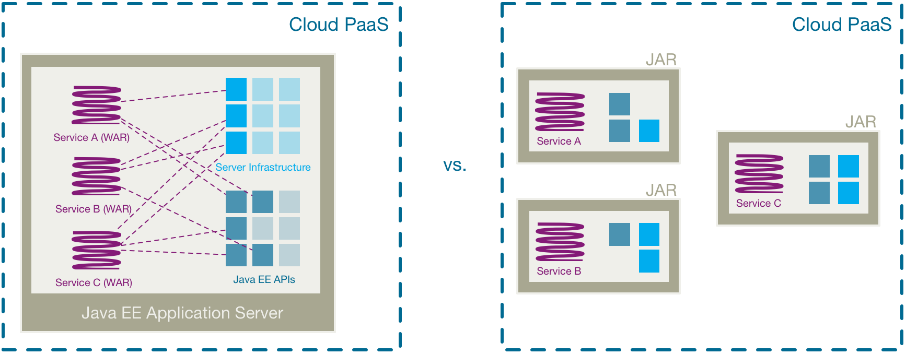
\includegraphics[width=1.0\linewidth]{images/mp}
	\caption{Bestandteile und Funktionalitäten im Service [1]}
	\label{fig:mp}
\end{figure}
Somit erhält man einen fachlich abgekapselten Service, der zudem seine eigene Laufzeitumgebung mit sich bringt. Diese Umgebung kann dabei entsprechend auf den Service angepasst werden, wodurch der Overhead hier auch drastisch reduziert werden kann. Sobald dieser Service nun deployt wird, kann er gestartet und ausgeführt werden. Er ist autark und läuft als eigener Prozess. Allerdings ist dieser Ansatz noch etwas zu grobgranular. Man kann hier von einem Self-contained System (SCS) sprechen [1]. Dieser Ansatz teilt sich zwar eine Vielzahl von Konzepten mit Microservices (Isolation, unabhängige Einheiten, fachliche Trennung, Technologiefreiheit, keine zentrale Infrastruktur), besitzt jedoch noch einige Unterschiede zum feingranularen Ansatz der Microservices. Wie eben bereits hervorgegangen ist, ist bereits die Größe ein Unterschied. Ein System besitzt normalerweise weniger SCS als Microservices. Ein wichtiger Aspekt ist die Kommunikation zwischen den Komponenten. Microservices können untereinander kommunizieren. SCSs sollten dies idealerweise nicht. Auch bringen Microservices oft ihre eigene Benutzeroberfläche mit sich, während sich SCSs eine gemeinsame teilen. Es wird an dieser Stelle also nicht das gewünschte Problem gelöst. SCSs sind eher für Architekturen größerer Projekte gedacht [3]. Sollen noch unabhängigere, kleinere Komponenten entwickelt werden, die auch mit Continuous Delivery arbeiten, muss noch ein Schritt weitergegangen werden. 
 
\section{MicroProfile}
Optimierungen erfolgen bisher durch recht triviale Ansätze. Ist der Anwendungsserver zu groß werden lediglich die benötigten Komponenten verwendet, die zwingend für den Microservice gebraucht werden. Diese Ansätze haben allerdings immer noch Schwachstellen, wie bereits aus dem obigen Kapitel hervorgegangen ist. Java EE MicroProfile wurde somit angekündigt, welches bei seiner initialen Version lediglich einen minimalen Satz an APIs zur Verfügung stellt. Somit enthielt die erste Version von MicroProfile JAX-RS für die Verwendung von REST, CDI und JSON-P. Dies reichte für einen Microservice ohne eigene Benutzeroberfläche aus. Bei Bedarf können zusätzliche APIs hinzugefügt werden. \\ \\
...